\everymath{\displaystyle}
\documentclass{beamer}
% \documentclass[handout]{beamer}

%\usepackage[pdftex]{color,graphicx}
\usepackage{amsmath,amssymb,amsfonts}

\mode<presentation>
{
  % \usetheme{Darmstadt}
  % \usetheme[hideothersubsections]{Hannover}
  % \usetheme[hideothersubsections]{Goettingen}
  \usetheme[hideothersubsections, right]{Berkeley}

  \usecolortheme{seahorse}
  % \usecolortheme{dolphin}
  \usecolortheme{rose}
  % \usecolortheme{orchid}

  \useinnertheme[shadow]{rounded}

  % \setbeamercovered{transparent}
  \setbeamercovered{invisible}
  % or whatever (possibly just delete it)
}

\mode<handout>{
  \setbeamercolor{background canvas}{bg=black!5}
  \usepackage{pgfpages}
  \pgfpagesuselayout{4 on 1}[a4paper,border shrink=5mm, landscape]
}

\usepackage[brazilian]{babel}
% or whatever

% \usepackage[latin1]{inputenc}
\usepackage[utf8]{inputenc}
% or whatever

\usepackage{times}
%\usepackage[T1]{fontenc}
% Or whatever. Note that the encoding and the font should match. If T1
% does not look nice, try deleting the line with the fontenc.


\title[Encerramento] % (optional, use only with long paper titles)
{Encerramento}

\subtitle
{Até mais, e obrigado pelo peixe} % (optional)

\author%[] % (optional, use only with lots of authors)
{Felipe Figueiredo}% \and S.~Another\inst{2}}
% - Use the \inst{?} command only if the authors have different
%   affiliation.

\institute[] % (optional, but mostly needed)
{
}
  % \inst{1}%
  % Department of Computer Science\\
  % University of Somewhere
  % \and
  % \inst{2}%
  % Department of Theoretical Philosophy\\
  % University of Elsewhere}
% - Use the \inst command only if there are several affiliations.
% - Keep it simple, no one is interested in your street address.

\date%[] % (optional)
{}

% \subject{Talks}
% This is only inserted into the PDF information catalog. Can be left
% out. 



% If you have a file called "university-logo-filename.xxx", where xxx
% is a graphic format that can be processed by latex or pdflatex,
% resp., then you can add a logo as follows:

\pgfdeclareimage[height=1.6cm]{university-logo}{../logo}
\logo{\pgfuseimage{university-logo}}



% Delete this, if you do not want the table of contents to pop up at
% the beginning of each subsection:
\AtBeginSubsection[]
%\AtBeginSection[]
{
  \begin{frame}<beamer>{Sumário}
    \tableofcontents[currentsection,currentsubsection]
  \end{frame}
}


% If you wish to uncover everything in a step-wise fashion, uncomment
% the following command: 

% \beamerdefaultoverlayspecification{<+->}

\usepackage[normalem]{ulem}

\begin{document}

\begin{frame}
  \titlepage
\end{frame}

\begin{frame}{Sumário}
  \tableofcontents
  % You might wish to add the option [pausesections]
\end{frame}


%% Template
% \section{}

% \subsection{}

% \begin{frame}{}
%   \begin{itemize}
%   \item 
%   \end{itemize}
% \end{frame}

% \begin{frame}
%   \begin{columns}
%     \begin{column}{5cm}
%     \end{column}
%     \begin{column}{5cm}
%     \end{column}
%   \end{columns}
% \end{frame}

% \begin{frame}{}
%   \includegraphics[height=0.4\textheight]{file1}
%   \includegraphics[height=0.4\textheight]{file2}
%   \includegraphics[height=0.4\textheight]{file3}
%   \begin{figure}
%     \caption{}
%   \end{figure}
% \end{frame}

% \begin{frame}{}
%   \begin{definition}
%   \end{definition}
%   \begin{example}
%   \end{example}
%   \begin{block}{Exercício}
%   \end{block}
% \end{frame}

\begin{frame}{A temporada até aqui}
  \begin{center}
    
\includegraphics[width=\textwidth]{Encerramento/theroadsofar}
  \end{center}
\end{frame}

\begin{frame}{Muito conteúdo}
  \begin{enumerate}
    \scriptsize
  \item Reprodutibilidade de estudos, e indicadores na Ciência
  \item Métodos Científicos, desenhos de estudo mais comuns e guidelines
  \item Problema, Hipótese, Variável
  \item Tópicos em Escrita Científica
  \item Revisão bibliográfica e Resumo
  \item Planejamento da pesquisa e eventuais fracassos
  \item Tópicos em Busca Bibliográfica (Google-fu, et al)
  \item Citações, Referências e Plágio (tutorial de referências no Mendeley)
  \item Estrutura I - Conteúdo das seções
  \item Estrutura II – Forma (tutorial de estilos no Word)
  \item Tópicos em resultados preliminares
  \item Tópicos em Estratégias de Apresentação
  \end{enumerate}
\end{frame}

\begin{frame}
  \begin{center}
    \Large

    Sempre que você publica...

    \bigskip
    \bigskip
    ... está se expondo a críticas
  \end{center}
\end{frame}

\begin{frame}{\tiny Para pensar: debate científico -- 1/3 -- artigo original}
  \begin{center}
    
\includegraphics[width=\textwidth]{Encerramento/polemica1}
  \end{center}
\end{frame}

\begin{frame}{\tiny Para pensar: debate científico -- 2/3 -- crítica}
  \begin{center}
    
\includegraphics[width=\textwidth]{Encerramento/polemica2}
  \end{center}
\end{frame}

\begin{frame}{\tiny Para pensar: debate científico -- 3/3 -- réplica}
  \begin{center}
    
\includegraphics[width=\textwidth]{Encerramento/polemica3}
  \end{center}
\end{frame}

\begin{frame}{\tiny Para pensar: debate científico -- 4/3 -- nunca se sabe quando termina!}
  \begin{center}
    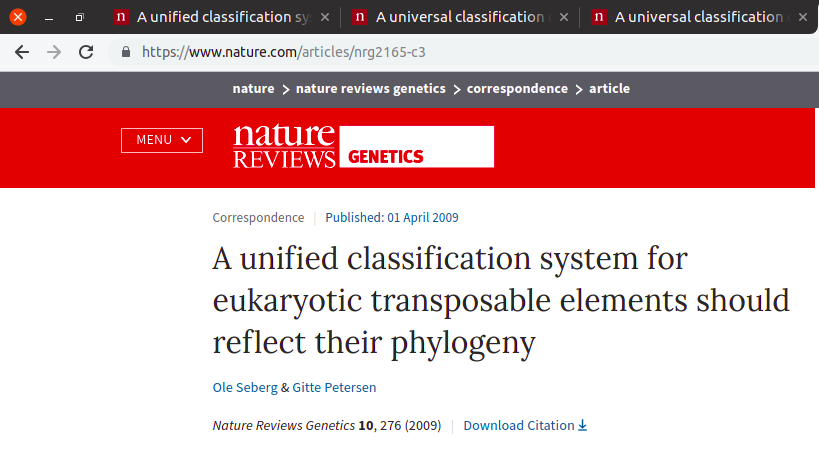
\includegraphics[width=\textwidth]{Encerramento/polemica4}
  \end{center}
\end{frame}

\begin{frame}{\tiny Para pensar: debate científico -- 5/3 -- nunca se sabe quando termina!}
  \begin{center}
    
\includegraphics[width=\textwidth]{Encerramento/polemica5}
  \end{center}
\end{frame}

\begin{frame}
  \begin{center}
    O processo científico...

    \bigskip
    \bigskip
    ... é a seleção natural das ideias.
  \end{center}
\end{frame}

\end{document}
